% Options for packages loaded elsewhere
\PassOptionsToPackage{unicode}{hyperref}
\PassOptionsToPackage{hyphens}{url}
\PassOptionsToPackage{dvipsnames,svgnames,x11names}{xcolor}
%
\documentclass[
  11pt,
  a4paper,
  DIV=11,
  numbers=noendperiod]{scrartcl}

\usepackage{amsmath,amssymb}
\usepackage{iftex}
\ifPDFTeX
  \usepackage[T1]{fontenc}
  \usepackage[utf8]{inputenc}
  \usepackage{textcomp} % provide euro and other symbols
\else % if luatex or xetex
  \usepackage{unicode-math}
  \defaultfontfeatures{Scale=MatchLowercase}
  \defaultfontfeatures[\rmfamily]{Ligatures=TeX,Scale=1}
\fi
\usepackage{lmodern}
\ifPDFTeX\else  
    % xetex/luatex font selection
\fi
% Use upquote if available, for straight quotes in verbatim environments
\IfFileExists{upquote.sty}{\usepackage{upquote}}{}
\IfFileExists{microtype.sty}{% use microtype if available
  \usepackage[]{microtype}
  \UseMicrotypeSet[protrusion]{basicmath} % disable protrusion for tt fonts
}{}
\makeatletter
\@ifundefined{KOMAClassName}{% if non-KOMA class
  \IfFileExists{parskip.sty}{%
    \usepackage{parskip}
  }{% else
    \setlength{\parindent}{0pt}
    \setlength{\parskip}{6pt plus 2pt minus 1pt}}
}{% if KOMA class
  \KOMAoptions{parskip=half}}
\makeatother
\usepackage{xcolor}
\usepackage[margin=1in]{geometry}
\setlength{\emergencystretch}{3em} % prevent overfull lines
\setcounter{secnumdepth}{5}
% Make \paragraph and \subparagraph free-standing
\makeatletter
\ifx\paragraph\undefined\else
  \let\oldparagraph\paragraph
  \renewcommand{\paragraph}{
    \@ifstar
      \xxxParagraphStar
      \xxxParagraphNoStar
  }
  \newcommand{\xxxParagraphStar}[1]{\oldparagraph*{#1}\mbox{}}
  \newcommand{\xxxParagraphNoStar}[1]{\oldparagraph{#1}\mbox{}}
\fi
\ifx\subparagraph\undefined\else
  \let\oldsubparagraph\subparagraph
  \renewcommand{\subparagraph}{
    \@ifstar
      \xxxSubParagraphStar
      \xxxSubParagraphNoStar
  }
  \newcommand{\xxxSubParagraphStar}[1]{\oldsubparagraph*{#1}\mbox{}}
  \newcommand{\xxxSubParagraphNoStar}[1]{\oldsubparagraph{#1}\mbox{}}
\fi
\makeatother

\usepackage{color}
\usepackage{fancyvrb}
\newcommand{\VerbBar}{|}
\newcommand{\VERB}{\Verb[commandchars=\\\{\}]}
\DefineVerbatimEnvironment{Highlighting}{Verbatim}{commandchars=\\\{\}}
% Add ',fontsize=\small' for more characters per line
\usepackage{framed}
\definecolor{shadecolor}{RGB}{241,243,245}
\newenvironment{Shaded}{\begin{snugshade}}{\end{snugshade}}
\newcommand{\AlertTok}[1]{\textcolor[rgb]{0.68,0.00,0.00}{#1}}
\newcommand{\AnnotationTok}[1]{\textcolor[rgb]{0.37,0.37,0.37}{#1}}
\newcommand{\AttributeTok}[1]{\textcolor[rgb]{0.40,0.45,0.13}{#1}}
\newcommand{\BaseNTok}[1]{\textcolor[rgb]{0.68,0.00,0.00}{#1}}
\newcommand{\BuiltInTok}[1]{\textcolor[rgb]{0.00,0.23,0.31}{#1}}
\newcommand{\CharTok}[1]{\textcolor[rgb]{0.13,0.47,0.30}{#1}}
\newcommand{\CommentTok}[1]{\textcolor[rgb]{0.37,0.37,0.37}{#1}}
\newcommand{\CommentVarTok}[1]{\textcolor[rgb]{0.37,0.37,0.37}{\textit{#1}}}
\newcommand{\ConstantTok}[1]{\textcolor[rgb]{0.56,0.35,0.01}{#1}}
\newcommand{\ControlFlowTok}[1]{\textcolor[rgb]{0.00,0.23,0.31}{\textbf{#1}}}
\newcommand{\DataTypeTok}[1]{\textcolor[rgb]{0.68,0.00,0.00}{#1}}
\newcommand{\DecValTok}[1]{\textcolor[rgb]{0.68,0.00,0.00}{#1}}
\newcommand{\DocumentationTok}[1]{\textcolor[rgb]{0.37,0.37,0.37}{\textit{#1}}}
\newcommand{\ErrorTok}[1]{\textcolor[rgb]{0.68,0.00,0.00}{#1}}
\newcommand{\ExtensionTok}[1]{\textcolor[rgb]{0.00,0.23,0.31}{#1}}
\newcommand{\FloatTok}[1]{\textcolor[rgb]{0.68,0.00,0.00}{#1}}
\newcommand{\FunctionTok}[1]{\textcolor[rgb]{0.28,0.35,0.67}{#1}}
\newcommand{\ImportTok}[1]{\textcolor[rgb]{0.00,0.46,0.62}{#1}}
\newcommand{\InformationTok}[1]{\textcolor[rgb]{0.37,0.37,0.37}{#1}}
\newcommand{\KeywordTok}[1]{\textcolor[rgb]{0.00,0.23,0.31}{\textbf{#1}}}
\newcommand{\NormalTok}[1]{\textcolor[rgb]{0.00,0.23,0.31}{#1}}
\newcommand{\OperatorTok}[1]{\textcolor[rgb]{0.37,0.37,0.37}{#1}}
\newcommand{\OtherTok}[1]{\textcolor[rgb]{0.00,0.23,0.31}{#1}}
\newcommand{\PreprocessorTok}[1]{\textcolor[rgb]{0.68,0.00,0.00}{#1}}
\newcommand{\RegionMarkerTok}[1]{\textcolor[rgb]{0.00,0.23,0.31}{#1}}
\newcommand{\SpecialCharTok}[1]{\textcolor[rgb]{0.37,0.37,0.37}{#1}}
\newcommand{\SpecialStringTok}[1]{\textcolor[rgb]{0.13,0.47,0.30}{#1}}
\newcommand{\StringTok}[1]{\textcolor[rgb]{0.13,0.47,0.30}{#1}}
\newcommand{\VariableTok}[1]{\textcolor[rgb]{0.07,0.07,0.07}{#1}}
\newcommand{\VerbatimStringTok}[1]{\textcolor[rgb]{0.13,0.47,0.30}{#1}}
\newcommand{\WarningTok}[1]{\textcolor[rgb]{0.37,0.37,0.37}{\textit{#1}}}

\providecommand{\tightlist}{%
  \setlength{\itemsep}{0pt}\setlength{\parskip}{0pt}}\usepackage{longtable,booktabs,array}
\usepackage{calc} % for calculating minipage widths
% Correct order of tables after \paragraph or \subparagraph
\usepackage{etoolbox}
\makeatletter
\patchcmd\longtable{\par}{\if@noskipsec\mbox{}\fi\par}{}{}
\makeatother
% Allow footnotes in longtable head/foot
\IfFileExists{footnotehyper.sty}{\usepackage{footnotehyper}}{\usepackage{footnote}}
\makesavenoteenv{longtable}
\usepackage{graphicx}
\makeatletter
\def\maxwidth{\ifdim\Gin@nat@width>\linewidth\linewidth\else\Gin@nat@width\fi}
\def\maxheight{\ifdim\Gin@nat@height>\textheight\textheight\else\Gin@nat@height\fi}
\makeatother
% Scale images if necessary, so that they will not overflow the page
% margins by default, and it is still possible to overwrite the defaults
% using explicit options in \includegraphics[width, height, ...]{}
\setkeys{Gin}{width=\maxwidth,height=\maxheight,keepaspectratio}
% Set default figure placement to htbp
\makeatletter
\def\fps@figure{htbp}
\makeatother
% definitions for citeproc citations
\NewDocumentCommand\citeproctext{}{}
\NewDocumentCommand\citeproc{mm}{%
  \begingroup\def\citeproctext{#2}\cite{#1}\endgroup}
\makeatletter
 % allow citations to break across lines
 \let\@cite@ofmt\@firstofone
 % avoid brackets around text for \cite:
 \def\@biblabel#1{}
 \def\@cite#1#2{{#1\if@tempswa , #2\fi}}
\makeatother
\newlength{\cslhangindent}
\setlength{\cslhangindent}{1.5em}
\newlength{\csllabelwidth}
\setlength{\csllabelwidth}{3em}
\newenvironment{CSLReferences}[2] % #1 hanging-indent, #2 entry-spacing
 {\begin{list}{}{%
  \setlength{\itemindent}{0pt}
  \setlength{\leftmargin}{0pt}
  \setlength{\parsep}{0pt}
  % turn on hanging indent if param 1 is 1
  \ifodd #1
   \setlength{\leftmargin}{\cslhangindent}
   \setlength{\itemindent}{-1\cslhangindent}
  \fi
  % set entry spacing
  \setlength{\itemsep}{#2\baselineskip}}}
 {\end{list}}
\usepackage{calc}
\newcommand{\CSLBlock}[1]{\hfill\break\parbox[t]{\linewidth}{\strut\ignorespaces#1\strut}}
\newcommand{\CSLLeftMargin}[1]{\parbox[t]{\csllabelwidth}{\strut#1\strut}}
\newcommand{\CSLRightInline}[1]{\parbox[t]{\linewidth - \csllabelwidth}{\strut#1\strut}}
\newcommand{\CSLIndent}[1]{\hspace{\cslhangindent}#1}

\KOMAoption{captions}{tableheading,figureheading}
\makeatletter
\@ifpackageloaded{caption}{}{\usepackage{caption}}
\AtBeginDocument{%
\ifdefined\contentsname
  \renewcommand*\contentsname{Table of contents}
\else
  \newcommand\contentsname{Table of contents}
\fi
\ifdefined\listfigurename
  \renewcommand*\listfigurename{List of Figures}
\else
  \newcommand\listfigurename{List of Figures}
\fi
\ifdefined\listtablename
  \renewcommand*\listtablename{List of Tables}
\else
  \newcommand\listtablename{List of Tables}
\fi
\ifdefined\figurename
  \renewcommand*\figurename{Figure}
\else
  \newcommand\figurename{Figure}
\fi
\ifdefined\tablename
  \renewcommand*\tablename{Table}
\else
  \newcommand\tablename{Table}
\fi
}
\@ifpackageloaded{float}{}{\usepackage{float}}
\floatstyle{ruled}
\@ifundefined{c@chapter}{\newfloat{codelisting}{h}{lop}}{\newfloat{codelisting}{h}{lop}[chapter]}
\floatname{codelisting}{Listing}
\newcommand*\listoflistings{\listof{codelisting}{List of Listings}}
\makeatother
\makeatletter
\makeatother
\makeatletter
\@ifpackageloaded{caption}{}{\usepackage{caption}}
\@ifpackageloaded{subcaption}{}{\usepackage{subcaption}}
\makeatother

\ifLuaTeX
  \usepackage{selnolig}  % disable illegal ligatures
\fi
\usepackage{bookmark}

\IfFileExists{xurl.sty}{\usepackage{xurl}}{} % add URL line breaks if available
\urlstyle{same} % disable monospaced font for URLs
\hypersetup{
  pdftitle={Menu Engineering Supercharged},
  pdfauthor={Hankun Xiao, Yasmin Hassan, Jessie Zhang, Zhiwei Zhang},
  colorlinks=true,
  linkcolor={blue},
  filecolor={Maroon},
  citecolor={Blue},
  urlcolor={Blue},
  pdfcreator={LaTeX via pandoc}}


\title{Menu Engineering Supercharged}
\usepackage{etoolbox}
\makeatletter
\providecommand{\subtitle}[1]{% add subtitle to \maketitle
  \apptocmd{\@title}{\par {\large #1 \par}}{}{}
}
\makeatother
\subtitle{MDS Capstone Technical Report}
\author{Hankun Xiao, Yasmin Hassan, Jessie Zhang, Zhiwei Zhang}
\date{}

\begin{document}
\maketitle

\renewcommand*\contentsname{Table of contents}
{
\hypersetup{linkcolor=}
\setcounter{tocdepth}{2}
\tableofcontents
}

\section{Introduction}\label{introduction}

This technical report serves as a behind-the-scenes narrative of our
capstone project for Heymate!. It documents how we tackled technical
challenges and highlights key decisions made during development and
deployment. It also provides a reference for future development.

\section{User Requirement Collection and Solution
Consulting}\label{user-requirement-collection-and-solution-consulting}

This capstone project with Heymate! differed from typical capstone
projects. Usually, the project partner provides specific objectives for
the deliverable as well as the dataset. In the project proposal from
Heymate!, they expected our data output as a dashboard to improve
customer retention. However, at the beginning of the project, we did not
receive a useful dataset.

Given this situation, we had a two-hour meeting with the partner to
understand their business needs and consult on potential solutions. We
received clarification that the partner actually wanted a \textbf{menu
recommendation model} (``the recommendation model'') for their clients
(restaurant owners). For example, one of Heymate!'s clients, a Chinese
Restaurant in Vancouver, wanted recommendations on what items to add and
what items to remove, following marketing trends.

Correspondingly, we agreed with the project partner and the project
supervisor that we would shift the project from ``Customer Retention
Supercharged'' to ``\textbf{Menu Engineering Supercharged},'' and we
agreed upon the techinical deliverables:

\begin{itemize}
\tightlist
\item
  A data cleaning module that can clean menu data and extract key
  features.
\item
  A knowledge base (database table) with proper schema design and
  initial data.
\item
  A recommendation algorithm.
\item
  A visualization demo for reference.
\end{itemize}

\section{Preparing the Dataset}\label{preparing-the-dataset}

To build the recommendation model, we needed training data. We compared
several datasets shared by the partner, our advisor, and our own
research:

\begin{itemize}
\tightlist
\item
  \textbf{Dothub Dataset Shared by the Partner:} This dataset is 66.4 GB
  and consists of 6,479,347 rows, including restaurant names and
  addresses in the US DoltHub (2022). We didn't choose this dataset
  because it did not include restaurant menu data.
\item
  \textbf{Yelp Dataset Shared by the Partner:} This dataset includes
  6,990,280 reviews from 150,346 restaurants Yelp (2025). While
  restaurant reviews could potentially be a good feature for building
  the model, it lacked menu data. This limitation made it unsuitable for
  direct use.
\item
  \textbf{What's On The Menu? Dataset by New York Public Library:} This
  dataset includes about 45,000 menus from the 1840s to 2016, containing
  restaurant information and menu data New York Public Library (2019).
  However, the dataset is old and doesn't necessarily reflect the most
  up-to-date trends, so we didn't choose it.
\item
  \textbf{Uber Eats Dataset (``the Uber Eats Data''):} This dataset
  includes over 63,000 restaurants and more than 5 million menus from
  Uber Eats in the US, collected in 2023 Sakib (2023). It contains
  restaurant names, review information, and individual menu items. Due
  to its recency and completeness, we agreed on this dataset with the
  partner.
\end{itemize}

\section{Dataset EDA and Feature
Engineering}\label{dataset-eda-and-feature-engineering}

Given the nature of the data, there were missing values, spelling
mistakes, variations, and language differences. We needed to apply
methods to clean the data and perform necessary feature engineering
before proceeding with the analysis.

For feature engineering, we aimed to extract \textbf{dish base} and
\textbf{dish flavors} from the item name, category, and descriptions in
the menu. Here is an example:

\begin{quote}
\textbf{Original Menu Item:} ``Classic Cheeseburger''\\
\textbf{Category:} ``Classic Burgers''\\
\textbf{Description:} ``Smashed beef patty with cheddar cheese and your
choice of toppings and sauce.''

\textbf{Extracted Features:}\\
- \textbf{Dish Base:} Burger\\
- \textbf{Dish Flavors:} Cheese, Beef
\end{quote}

We considered the following approaches:

\begin{itemize}
\tightlist
\item
  \textbf{Regular Expressions:} Regular expressions are effective for
  processing data with consistent patterns. However, in our data, each
  restaurant had its own preference for writing the menu, making this
  method inconsistent for universal application.
\item
  \textbf{An Existing Word Embedding Model from HuggingFace, Specialized
  with Menu Corpus:} This method was suggested by Professor Verada, who
  specializes in machine learning within the UBC MDS teaching team.
  Unfortunately, the Uber Eats data contained information in different
  languages, and we couldn't find a suitable multi-language model from
  HuggingFace.
\item
  \textbf{A Generalized Large Language Model (LLM):} This method
  involves using an external LLM to clean the data. We added specific
  instructions through prompt engineering on how the data should be
  cleaned and engineered. The processed data was then retrieved from the
  model. Additionally, the partner shared their organization's ChatGPT
  subscription with us and provided API tokens. After balancing cost and
  efficiency, we chose the \textbf{GPT-4o mini model}.
\end{itemize}

Here is a table comparing the different approaches:

\begin{longtable}[]{@{}
  >{\raggedright\arraybackslash}p{(\columnwidth - 4\tabcolsep) * \real{0.2569}}
  >{\raggedright\arraybackslash}p{(\columnwidth - 4\tabcolsep) * \real{0.4861}}
  >{\raggedright\arraybackslash}p{(\columnwidth - 4\tabcolsep) * \real{0.2569}}@{}}
\toprule\noalign{}
\begin{minipage}[b]{\linewidth}\raggedright
Approach
\end{minipage} & \begin{minipage}[b]{\linewidth}\raggedright
Pros
\end{minipage} & \begin{minipage}[b]{\linewidth}\raggedright
Cons
\end{minipage} \\
\midrule\noalign{}
\endhead
\bottomrule\noalign{}
\endlastfoot
Regular Expressions & Fast to compute; Free & Limited flexibility \\
& & \\
Existing Word Embedding Model (HuggingFace) & Semantic understanding;
Efficiency; Free & Multi-lingual challenge \\
& & \\
Generalized Large Language Model (LLM) & Highly flexible; Supporting
Multi-lingual; Semantic understanding & Costly; Slow; API Reliance \\
\end{longtable}

\section{Research on the Recommendation
Algorithm}\label{research-on-the-recommendation-algorithm}

We researched three common recommendation methods used in the industry:
\textbf{Collaborative Filtering}, \textbf{Content-Based Filtering}, and
\textbf{Popularity-Based Recommendation}.

\begin{itemize}
\tightlist
\item
  \textbf{Collaborative Filtering / Matrix Factorization:} This method
  is widely used in industry, including by companies like Netflix, to
  generate recommendations based on user-item interaction data (e.g.,
  purchase history or user ratings) Gomez-Uribe and Hunt (2016).
  However, in the Uber Eats dataset, we do not have access to such user
  interaction data, making this method infeasible for our use case.
\item
  \textbf{Content-Based Filtering with Vector Embeddings:} This involves
  using a pre-trained large language model to convert menu items from
  human-readable text into numeric vectors. For example, ``Fried
  Chicken'' might be transformed into \([0.1, 0.5, 0.9]\), while ``Dim
  Sum'' could become \([0.2, 0.6, 0.1]\). These numeric representations
  allow us to quantify the similarities and differences between
  different cuisines, enabling further recommendations. Unfortunately,
  due to time and resource constraints, we were unable to deploy a large
  language model locally or fine-tune one.
\item
  \textbf{Popularity-Based Recommendation:} Popularity is a widely
  accepted baseline metric in the industry, used by platforms like Yelp
  Chitalia (2023), and GitHub Sreekala (2020). For instance, GitHub
  calculates a popularity score based on the number of forks a
  repository receives Al-Rubaye and Sukthankar (2020). For Heymate!, we
  designed a custom formula that incorporates the \textbf{number of
  reviews}, \textbf{average rating of a restaurant}, and the
  \textbf{frequency of a cuisine} to calculate a popularity score. These
  data points are available in the Uber Eats dataset. Additionally, this
  method is easy to understand and communicate to restaurant owners.
  Given its advantages in both interpretability and feasibility, we
  chose to adopt a \textbf{Popularity-Based Recommendation} approach in
  our project.
\end{itemize}

\section{Techinical Implemetation}\label{techinical-implemetation}

During development, the team utilized GitHub and Slack for communication
and collaboration. We modularized each component for future improvement.

\begin{itemize}
\tightlist
\item
  \href{https://github.com/UBC-MDS/heymate-report/blob/readme-update/script/visualization_demo.ipynb}{\texttt{visualization\_demo.ipynb}}:
  A notebook that visualizes the recommendation output.
\item
  \href{https://github.com/UBC-MDS/heymate-report/blob/readme-update/script/knowledge_base_update.ipynb}{\texttt{knowledge\_base\_update.ipynb}}:
  A notebook manages the task of updating the knowledge base of menu
  data.
\item
  \href{https://github.com/UBC-MDS/heymate-report/blob/readme-update/script/archived_function_app.py}{\texttt{archived\_function\_app.py}}:
  Stores deprecated Azure Function logic.
\item
  \href{https://github.com/UBC-MDS/heymate-report/blob/readme-update/script/batch_cleaning.py}{\texttt{batch\_cleaning.py}}:
  Cleans raw menu data in batches.
\item
  \href{https://github.com/UBC-MDS/heymate-report/blob/readme-update/script/credential_validation_test_unit.py}{\texttt{credential\_validation\_test\_unit.py}}:
  Unit tests for verifying database and API credentials.
\item
  \href{https://github.com/UBC-MDS/heymate-report/blob/readme-update/script/flask_deploy.py}{\texttt{flask\_deploy.py}}:
  Deploy the data cleaning module locally under the Flask framework.
\item
  \href{https://github.com/UBC-MDS/heymate-report/blob/readme-update/script/menu_recommender.py}{\texttt{menu\_recommender.py}}:
  Recommends menu items and return the output as a JSON object.
\item
  \href{https://github.com/UBC-MDS/heymate-report/blob/readme-update/script/popularity_score_calculator.py}{\texttt{popularity\_score\_calculator.py}}:
  Calculates popularity scores for items.
\item
  \href{https://github.com/UBC-MDS/heymate-report/blob/readme-update/script/util_database_reader.py}{\texttt{util\_database\_reader.py}}:
  Utility to read data from a database.
\item
  \href{https://github.com/UBC-MDS/heymate-report/blob/readme-update/script/util_database_uploader.py}{\texttt{util\_database\_uploader.py}}:
  Utility to upload or write data to a database.
\item
  \href{https://github.com/UBC-MDS/heymate-report/blob/readme-update/script/util_llm_data_cleaner.py}{\texttt{util\_llm\_data\_cleaner.py}}:
  Utility to send and retrieve the data to ChatGPT's API.
\item
  \href{https://github.com/UBC-MDS/heymate-report/blob/readme-update/script/util_task_logger.py}{\texttt{util\_task\_logger.py}}:
  Logs tasks or events during execution for tracking/debugging.
\end{itemize}

\section{Deployment of the Data Cleaning
Module}\label{deployment-of-the-data-cleaning-module}

\subsection{Research and Decision
Making}\label{research-and-decision-making}

Due to the numerous amount of data (3 million rows), we decided to
deploy the data cleaning module using a \textbf{distributed deployment
approach}. This means multiple working instances would clean batches
concurrently and run on cloud machines. We considered three approaches:

\begin{itemize}
\tightlist
\item
  \textbf{Google Cloud Function (part of Google Cloud Platform):} One
  team member had experience working with it in the past; however, the
  partner did not have a Google Cloud Subscription.
\item
  \textbf{Flask Function on an EC2 instance on Amazon Web Services
  (AWS):} This framework was introduced in the Cloud Computing Course
  during the MDS program. However, the partner did not have an AWS
  Subscription.
\item
  \textbf{Azure Function:} Azure Function is similar to Google Cloud
  Function, and working instances can be triggered via an HTTP web
  request. The partner had an Azure subscription and shared the
  credentials with us.
\end{itemize}

\subsection{Initial Deployment and
Blockers}\label{initial-deployment-and-blockers}

Given the cloud computing resources from the partner, we chose
\textbf{Azure Function} as our primary deployment plan. To automate the
deployment process, the team utilized the continuous deployment workflow
from GitHub by adding the following flow:

\begin{Shaded}
\begin{Highlighting}[]
\AttributeTok{  }\KeywordTok{{-}}\AttributeTok{ }\FunctionTok{name}\KeywordTok{:}\AttributeTok{ }\StringTok{\textquotesingle{}Deploy to Azure Functions\textquotesingle{}}
\AttributeTok{    }\FunctionTok{uses}\KeywordTok{:}\AttributeTok{ Azure/functions{-}action@v1}
\AttributeTok{    }\FunctionTok{id}\KeywordTok{:}\AttributeTok{ fa}
\AttributeTok{    }\FunctionTok{with}\KeywordTok{:}
\AttributeTok{      }\FunctionTok{app{-}name}\KeywordTok{:}\AttributeTok{ $\{\{ env.AZURE\_FUNCTIONAPP\_NAME \}\}}
\AttributeTok{      }\FunctionTok{package}\KeywordTok{:}\AttributeTok{ script}
\AttributeTok{      }\FunctionTok{publish{-}profile}\KeywordTok{:}\AttributeTok{ $\{\{ secrets.AZURE\_FUNCTIONAPP\_PUBLISH\_PROFILE \}\}}
\AttributeTok{      }\FunctionTok{scm{-}do{-}build{-}during{-}deployment}\KeywordTok{:}\AttributeTok{ }\CharTok{true}
\AttributeTok{      }\FunctionTok{enable{-}oryx{-}build}\KeywordTok{:}\AttributeTok{ }\CharTok{true}
\end{Highlighting}
\end{Shaded}

Unfortunately, the deployment failed due to security setup issues. The
partner had never used Azure Function before, and their engineers did
not have the time to configure the proper security settings for us. We
also did not want to risk compromising security, as the database stores
sensitive business and customer information.

\subsection{Alternative Deployment}\label{alternative-deployment}

We decided to deploy the data cleaning module locally on our computers
under the \textbf{Flask infrastructure}. We could still utilize the
distributed deployment framework to accelerate the process. With the
team's effort, we successfully cleaned:

\begin{itemize}
\tightlist
\item
  All of Heymate!'s internal menu database, including over 6,000
  entries.
\item
  More than 30,000 entries in the Uber Eats dataset.
\end{itemize}

This allowed us to proceed further with the implementation of the
recommendation alogorithm without blocking the project timeline.

\section{Onboarding Instruction and Suggestions for Future
Development}\label{onboarding-instruction-and-suggestions-for-future-development}

The developer should first install and activate the Conda environment
using the \texttt{environment.yml} file, and then set up the
\texttt{credentials} folder. More detailed instructions can be found
\href{https://github.com/UBC-MDS/heymate-report}{here}. Please note that
the ChatGPT API token is \textbf{not required} unless the developer
plans to load additional data into the knowledge base.

\href{https://github.com/UBC-MDS/heymate-report/blob/readme-update/script/visualization_demo.ipynb}{\texttt{visualization\_demo.ipynb}}
includes detailed instructions on how to trigger recommendations and
visualize the output. The developer can customize the visualization by
adjusting the Altair code and exporting the result as an HTML object. If
they would like to update the formula used for calculating the
popularity score, changes can be made in the
\href{https://github.com/UBC-MDS/heymate-report/blob/readme-update/script/popularity_score_calculator.py}{\texttt{popularity\_score\_calculator.py}}
script.

Currently, there are 30,000 data entries in the knowledge base, which
already provide decent results. If the developer wishes to load more
data, they can refer to the instructions in
\href{https://github.com/UBC-MDS/heymate-report/blob/readme-update/script/knowledge_base_update.ipynb}{\texttt{knowledge\_base\_update.ipynb}}.
To use a different LLM model, they can make the necessary changes in
\href{https://github.com/UBC-MDS/heymate-report/blob/readme-update/script/util_llm_data_cleaner.py}{\texttt{util\_llm\_data\_cleaner.py}}.

There are a few areas where this project could be extended:

\begin{itemize}
\tightlist
\item
  \textbf{Deployment of the Data Cleaning Module:} We currently deploy
  the code locally under the Flask framework. The code can be deployed
  as an Azure Function with proper setup. We provided
  \texttt{archived\_function\_app.py} as a reference code.
\item
  \textbf{Diverse Dataset:} We currently ingest only one dataset, the
  Uber Eats dataset. Potentially, more datasets could be added to enrich
  the recommendation model.
\item
  \textbf{Visualization Improvement:} We provided a demo visualization
  of the top recommended items Figure~\ref{fig-viz-demo}. When
  integrating the system into Heymate!'s restaurant management system,
  the developer should adjust the font and coloring to ensure that the
  visualization is coherent to the scheme.
\end{itemize}

\begin{figure}

\caption{\label{fig-viz-demo}Visualization Demo''}

\centering{

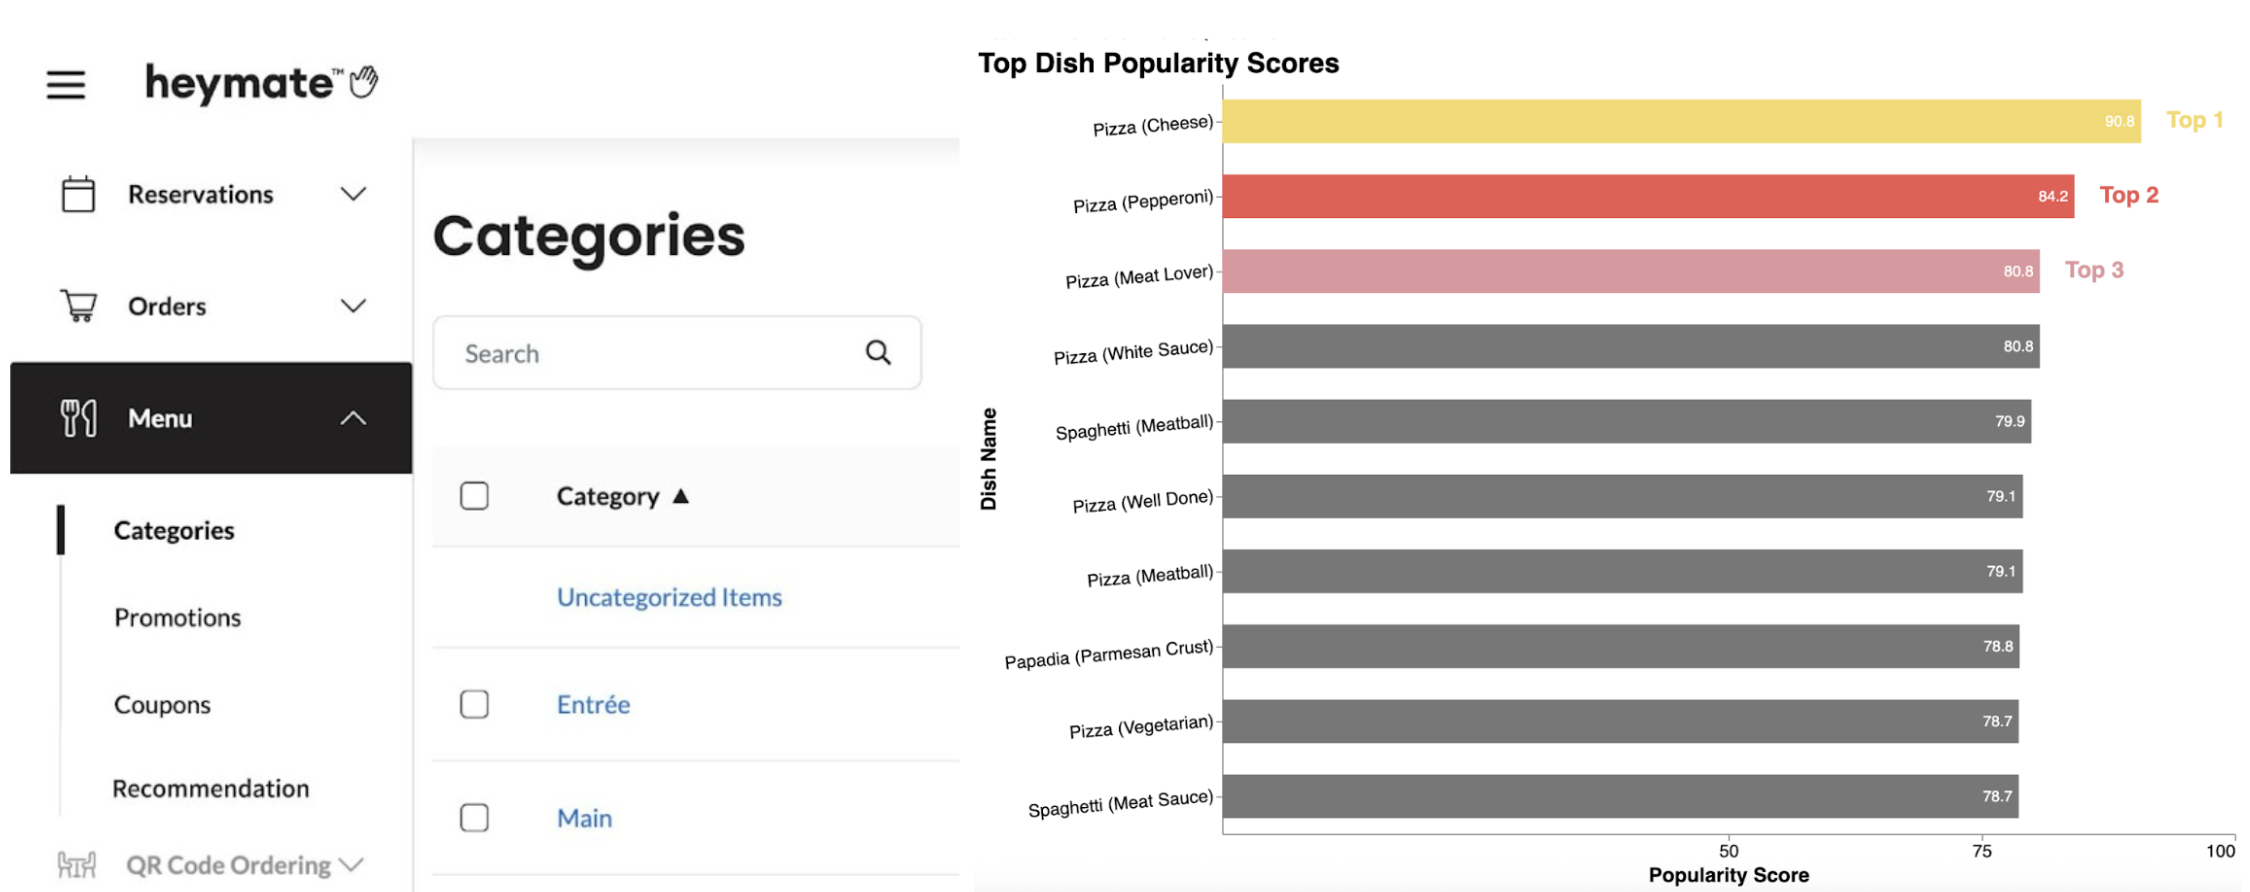
\includegraphics[width=0.8\textwidth,height=\textheight]{../image/final-8-viz.png}

}

\end{figure}%

\begin{itemize}
\tightlist
\item
  \textbf{Save cost on the LLM usage}: Save cost on LLM usage: To save
  costs in the long run, Heymate! can consider using an in-house local
  LLM such as Ollama. This can significantly reduce the usage cost of
  ChatGPT.
\end{itemize}

\newpage{}

\section*{References}\label{references}
\addcontentsline{toc}{section}{References}

\phantomsection\label{refs}
\begin{CSLReferences}{1}{0}
\bibitem[\citeproctext]{ref-alrubaye2020github}
Al-Rubaye, S., and G. Sukthankar. 2020. {``Popularity-Based Ranking of
GitHub Repositories.''} \emph{IEEE}.
\url{https://ieeexplore.ieee.org/document/9458206}.

\bibitem[\citeproctext]{ref-chitalia2023yelp}
Chitalia, A. 2023. {``Yelp Popularity Score Calculator.''}
\url{https://scholarworks.sjsu.edu/etd_projects/1261}.

\bibitem[\citeproctext]{ref-dolthub_menus}
DoltHub. 2022. {``Menus Dataset.''}
\url{https://www.dolthub.com/repositories/dolthub/menus/data/master}.

\bibitem[\citeproctext]{ref-gomezuribe2016netflix}
Gomez-Uribe, Carlos A., and Neil Hunt. 2016. {``The Netflix Recommender
System: Algorithms, Business Value, and Innovation.''} \emph{ACM
Transactions on Management Information Systems (TMIS)} 6 (4): 13:1--19.
\url{https://doi.org/10.1145/2843948}.

\bibitem[\citeproctext]{ref-nypl_menu}
New York Public Library. 2019. {``What's on the Menu? Dataset.''}
\url{https://www.kaggle.com/datasets/nypl/whats-on-the-menu/data}.

\bibitem[\citeproctext]{ref-ubereats_dataset}
Sakib, Ahmed Shahriar. 2023. {``Uber Eats USA Restaurants and Menus
Dataset.''}
\url{https://www.kaggle.com/datasets/ahmedshahriarsakib/uber-eats-usa-restaurants-menus/data}.

\bibitem[\citeproctext]{ref-sreekala2020popularity}
Sreekala, Keshetti. 2020. {``Popularity-Based Recommendation System.''}
\emph{ResearchGate}.

\bibitem[\citeproctext]{ref-yelp_open_dataset}
Yelp. 2025. {``Yelp Open Dataset.''}
\url{https://business.yelp.com/data/resources/open-dataset/}.

\end{CSLReferences}




\end{document}
